内点法的核心思想为通过迭代更新, 从多面体的内部逐渐接近最优解, 而不是像单纯形法那样沿着可行域的边界移动.

对于标准的线性规划问题
\optmodule*{\min}{\bm{c}^\mathrm{T}\bm{x}}{
    &\bm{Ax}=\bm{b}, \\
    &\bm{x}\geq\bm{0},
}
它的可行域为
\begin{equation*}
    \mathcal{F}=\{\bm{x} \mid \bm{Ax}=\bm{b}, \bm{x}\geq\bm{0}\}.
\end{equation*}

\begin{figure}[ht]
    \centering
    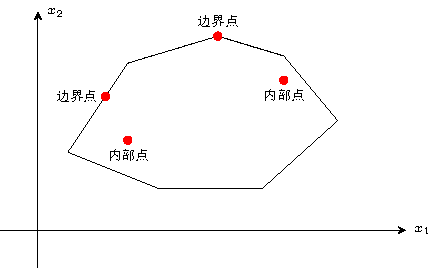
\includegraphics[scale=1.1]{figures/17-1.pdf}
    \caption{}
    \label{figure:17-1}
\end{figure}
如\cref{figure:17-1}所示, 可行域$\mathcal{F}$大致分为边界和内部.

\begin{figure}[ht]
    \centering
    \begin{subfigure}[c]{0.45\textwidth}
        \centering
        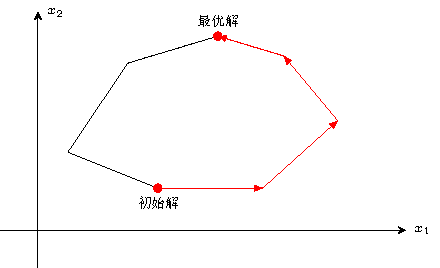
\includegraphics[width=0.9\textwidth]{figures/17-2.pdf}
        \caption{单纯形法}
        \label{figure:17-2}
    \end{subfigure}
    \begin{subfigure}[c]{0.45\textwidth}
        \centering
        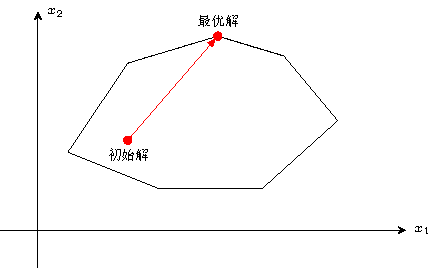
\includegraphics[width=0.9\textwidth]{figures/17-3.pdf}
        \caption{内点法}
        \label{figure:17-3}
    \end{subfigure}
    \caption{不同方法搜索过程示意图}
    \label{figure:search schematic}
\end{figure}

如\cref{figure:search schematic}所示, 单纯形法往往从多面体的一个顶点(基本可行解)出发, 沿着边界寻找最优解, 而内点法是从多面体的内部出发, 沿着搜索方向寻找最优解, 因此通常情况下, 内点法比单纯形法的效率更高.
